\documentclass[10pt,twocolumn,a4paper]{opticajnl}

\nonstopmode
\usepackage[utf8]{inputenc}
\usepackage[T1]{fontenc}


\usepackage[usefilenames,DefaultFeatures={Ligatures=Common}]{plex-otf} %
\usepackage{hyperref}
\usepackage{graphicx} 
\hypersetup{
    colorlinks=true,
    linkcolor=blue,
    filecolor=magenta,      
    urlcolor=purple,
    pdftitle={Proyecto Estancia Delfín - Renato Sanchez Loeza - 2024},
    }


\usepackage{listings}
\usepackage{color}
\definecolor{dkgreen}{rgb}{0,0.6,0}
\definecolor{gray}{rgb}{0.5,0.5,0.5}
\definecolor{mauve}{rgb}{0.58,0,0.82}

\lstset{
  frame=tb,
  language=Python,
  aboveskip=3mm,
  belowskip=3mm,
  showstringspaces=false,
  columns=flexible,
  basicstyle={\ttfamily\footnotesize},
  numbers=none,
  numberstyle=\tiny\color{gray},
  keywordstyle=\color{blue},
  commentstyle=\color{dkgreen},
  stringstyle=\color{mauve},
  breaklines=true,
  breakatwhitespace=true,
  tabsize=3,
}
\usepackage[style=apa,sorting=ynt]{biblatex}
\addbibresource{refs.bib}

\definecolor{color2}{RGB}{59,90,198} % author email, doi
\definecolor{color2b}{RGB}{105,105,105} % Header, authors, table lines

\title{Diagramas de diagnóstico en galaxias observadas con espectroscopía de campo MaNGA del Sloan Digital Sky Survey}
\author{Renato Sánchez Loeza - Estancia Verano 2024 Programa Delfín}

\begin{document}
\maketitle
\section*{Introducción}
Desde los inicios de la astronomía, nuestra visión del firmamento ha estado limitada por la capacidad tecnológica para observarlo. Pasando por etapas tempranas donde el ojo humano se apoyaba con los primeros telescopios ópticos para la definición de objetos celestes, tal como el holandés Hans Lippershey, quien construyó uno de los primeros telescopios en 1608, y Galileo Galilei, quien mejoró este modelo en 1610 \cite{cana-2015}.

Posteriormente, la fotografía mejoró la precisión de las mediciones. El primero en hacerlo fue John William Draper, quien en 1840 utilizó un proceso de daguerrotipo\footnote{Técnica fotográfica primitiva mediante la cual las imágenes captadas con la cámara oscura se fijan sobre una chapa metálica convenientemente preparada.} para capturar una imagen de la Luna. Cinco años más tarde, Foucault y Fizeau fotografiaron el Sol desde París \cite{olsen2021birth}. Pero los obstáculos se encuentran en la dificultad de compartir la información obtenida con base en este método.

Más recientemente, los CCD revolucionaron las observaciones astronómicas con una captura de entre el 90\% y el 95\% de la luz que llega a ellos, además de permitir la distribución de las fotografías obtenidas \cite{las-cumbres}. A estos avances se incorpora el análisis del espectro electromagnético (ondas de radio, infrarrojo, ultravioleta, rayos X y Gamma) y la espectroscopia, siendo la segunda la encargada de extraer datos sobre la distribución de la energía en una región del plano con el método de la rendija, donde por esta se permite entrar la luz del segmento a estudiar para posteriormente estudiar su espectrograma.

En la búsqueda de métodos que combinen lo mejor de la fotometría y la espectroscopia, se han propuesto diversas técnicas. Entre ellas, destacan el barrido con rendijas, el interferómetro de Fabry-Pérot (Etalon) y la espectroscopia multiobjetos (MOS). El barrido con rendijas implica observar la luz de una fuente a través de una rendija estrecha. Esto permite analizar su espectro y obtener información sobre composición química, velocidad y temperatura, mientras que el Fabry-Pérot es una técnica que utiliza múltiples reflexiones entre dos superficies altamente reflectantes y cercanas entre sí \cite{olmo-nave}. Por otro lado, la MOS emplea máscaras con múltiples aperturas para capturar espectros de varios objetos simultáneamente \cite{oconnell_astr511}, a menudo utilizando una matriz de fibras para capturar parte del campo de visión. Estas fibras se encuentran en el plano focal del instrumento de imagen. Luego, las fibras se redirigen y se alinean en la ranura de entrada del espectrógrafo, dispersando la luz en un detector. Se emplea en estudios de objetos débiles, como cúmulos de galaxias. Ejemplo de estos sistemas son el \textit{Low Resolution Imaging Spectrometer} (LRIS) en el Keck I y el \textit{VIsible MultiObject Spectrograph} (VIMOS) \footnote{“VIMOS operates in three different modes: Imaging (IMG), Multi-Object Spectroscopy (MOS), and with Integral Field Unit (IFU).” \cite{eso_vimos}} en el VLT \cite{oke_1995}.

\begin{figure}
    \centering
    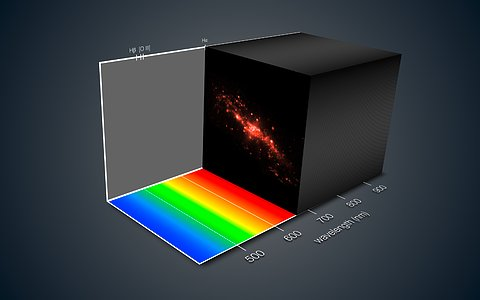
\includegraphics[width=0.8\linewidth]{ifus.jpg}
    \caption{Visualización de un cubo de datos resultante de una IFS. Crédito: ESO/MUSE consortium/R. Bacon/L. Calçada}
    \label{fig:ifus}
\end{figure}

\section*{Espectroscopia Integral de Campo}
Sin embargo, el sistema que hoy en día se usa con más frecuencia es la espectroscopia integral de campo o IFS (Integral Field Spectrograph), la cual nos permite obtener un espectrograma de una región de 2 dimensiones del espacio. Un IFS genera un cubo de datos (Fig. 1), que contiene el campo de visión en 2 dimensiones y una dimensión espectral, formado por un bloque de imágenes de la misma región, cada una en una longitud de onda diferente \cite{UW-Madison-IFS}. Los astrónomos pueden medir, por ejemplo, el movimiento del gas en una galaxia lejana o las distancias a las diferentes galaxias detectadas en un campo de visión, utilizando la riqueza de la información de los espectrógrafos de campo integral.

En este proceso se encuentran las Unidades Integrales de Campo o IFU (Integral Field Units), los cuales son ampliamente utilizados para estudiar objetos de gran extensión, como cúmulos, galaxias o nebulosas, en una sola toma. Durante este proceso, la señal de cada una de las celdas se procesa en un espectrógrafo, el cual genera un espectro para cada uno de los píxeles, generando así un \textit{spaxel}, y al final del proceso obtenemos un cubo de datos o \textit{datacube}.

\subsection*{Métodos de IFS}
\subsubsection*{Arreglo de lentes o Lenslet arrays}
Utiliza imágenes de pupila para distribuir espectros cortos. La magnificación y espacio entre espectros es importante para evitar mezcla de luz de diferentes longitudes de onda (Fig. 2) \cite{allington2006basic}.
\begin{figure}
    \centering
    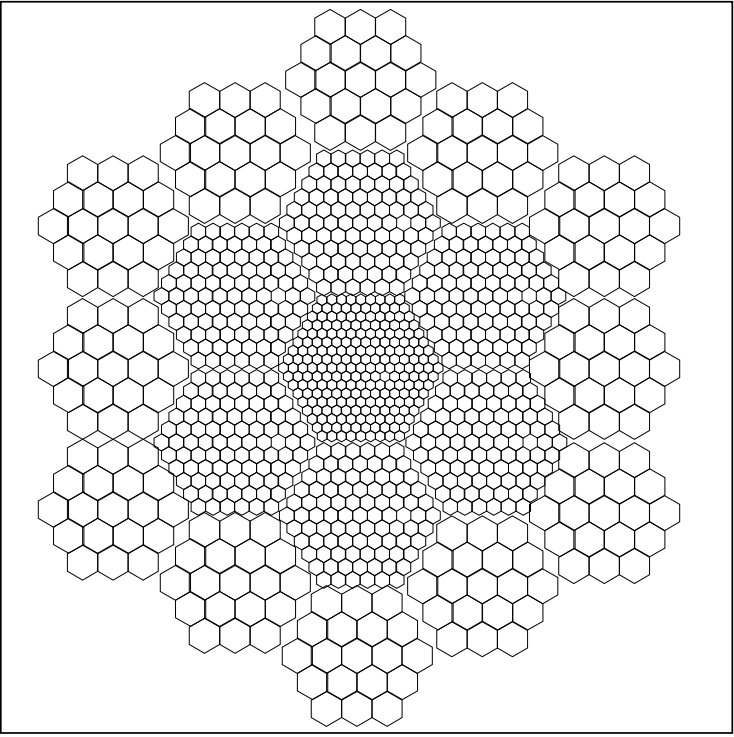
\includegraphics[width=0.8\linewidth]{lensletsimg1.png}
    \caption{Ejemplo de arreglo de lentes hexagonales con 3 tamaños de spaxels. Crédito: \cite{schmoll2006design}}
    \label{fig:lensletsimg1}
\end{figure}

\subsubsection*{Arreglo de fibras o Fibre arrays} 
Esta técnica consiste en acoplar una serie de fibras y un arreglo de microlentes \footnote{Los arreglos de microlentes son necesarios para las IFU acopladas a fibras. Adaptan el cono de luz entrante a la fibra, al mismo tiempo que optimizan el factor de llenado del conjunto de entrada. \cite{schmoll2006design}} que redirigen la luz a las rendijas para la generación de espectrogramas. Cada fibra recoge la luz de una ubicación específica en el campo de visión (Fig. 3). Además, requiere menos espacio muerto y, por lo tanto, tiene el potencial de aumentar la densidad de información \cite{allington2006basic}.
\begin{figure}
    \centering
    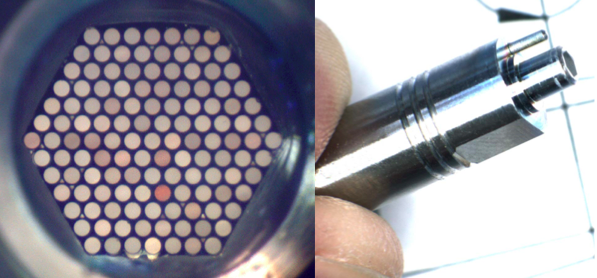
\includegraphics[width=0.8\linewidth]{fibrefeed.png}
    \caption{A la izquierda se muestra la cara del primer prototipo de IFU de 127 fibras. A la derecha se muestra la carcasa de la férula que sostiene la IFU y permite enchufarla a la placa SDSS. \cite{sdss_bundle_ferrule}}
    \label{fig:fibrefeed}
\end{figure}


\subsubsection*{Cortador o Slicer}
Un cortador de imágenes se compone generalmente de un conjunto de espejos cortadores ubicados en el plano de la imagen del telescopio y asociados a una fila de espejos pupilares y una fila de espejos de rendija \cite{vives2005original}. Esta técnica busca dividir la imagen en tiras para después dispersarlas y formar un espectro (Fig. 4).
\begin{figure}
    \centering
    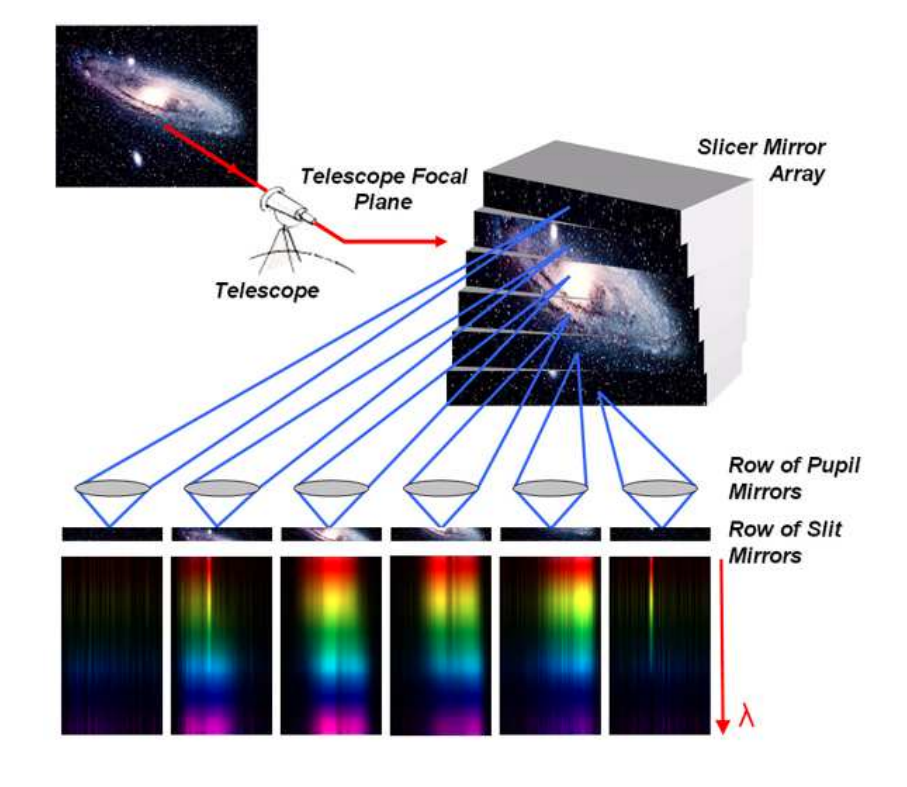
\includegraphics[width=1\linewidth]{slicerimg1.png}
    \caption{Visualización de un IFU Slicer. Crédito: \cite{vives2005original}}
    \label{fig:slicerimg1}
\end{figure}


\section*{Visualización y Análisis}
Si bien se ha avanzado significativamente en la mejora de nuestros métodos para observar las regiones espaciales, ahora es el momento de analizar dichos datos para obtener un aporte al conocimiento mucho más sofisticado. Hoy en día, podemos encontrar distintos software de procesamiento de datos de este tipo para modelos y usos muy específicos. Sin embargo, no podemos decir que exista una herramienta universal que nos brinde las herramientas suficientes para manipular datos de cualquier procedencia, con una interfaz intuitiva y una gran variedad de opciones para procesar los datos.

\subsection*{Soluciones existentes}
 \subsubsection*{Marvin}
Actualmente se encuentra disponible Marvin \cite{marvin}, un conjunto de herramientas que incluye un paquete de Python, una API y una aplicación web, diseñado para trabajar con los datos del proyecto MaNGA de SDSS-IV. Este software está equipado con datos generales de las galaxias, como las coordenadas celestes, la fecha de observación y una imagen de la galaxia observada, así como la visualización espectral en un spaxel específico (espectro observado y modelo de ajuste) con la opción de marcar los componentes químicos que refleja la espectroscopia. Incluye mapas de propiedades de la galaxia en cuestión, con datos como la velocidad estelar y el flujo de líneas de emisión \textbf{(Fig. 5)}.
\begin{figure}
	\centering
  	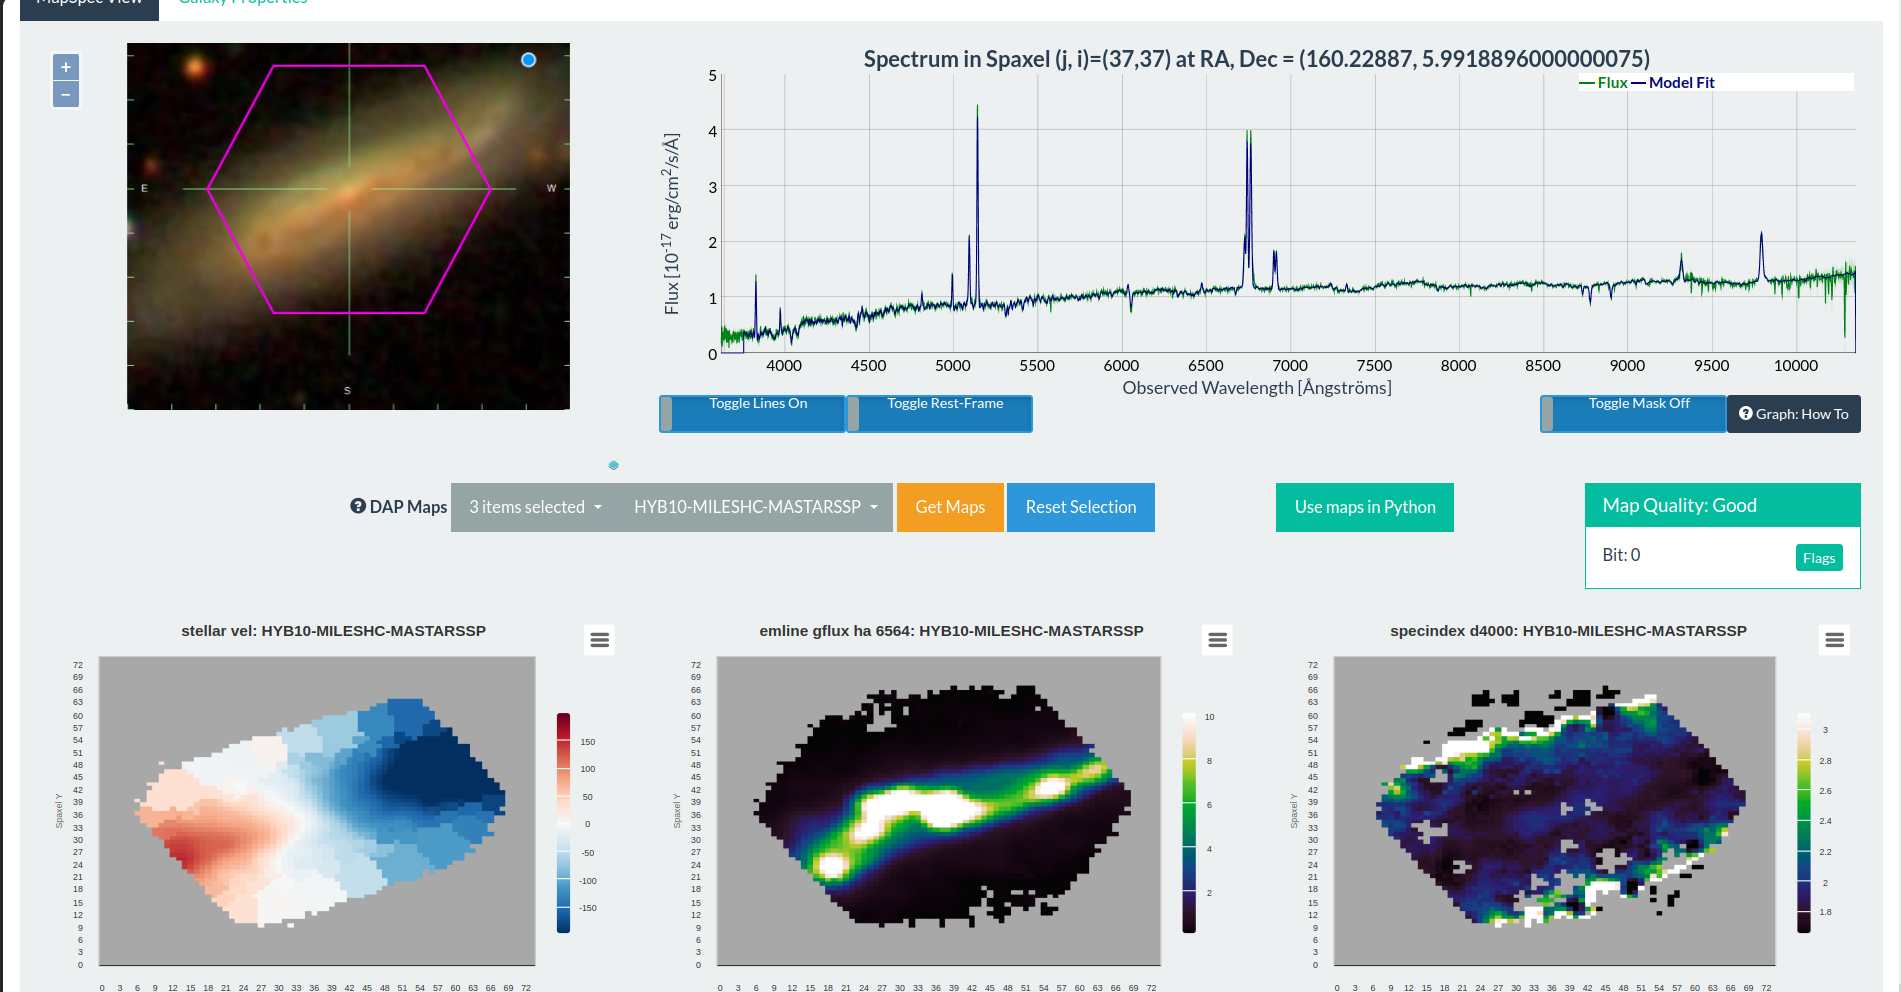
\includegraphics[width=0.8\linewidth]{interfaceMarvin}
	\caption{Interfaz web de Marvin.}
	\label{fig:interfacemarvin}
\end{figure}

\subsubsection*{Starlink}
También contamos con Starlink \cite{Berry_Starlink}, un proyecto de código abierto para el procesamiento de datos astronómicos. Aunque este proyecto terminó en 2005, el software sigue en desarrollo por la \textit{East Asian Observatory}. Una desventaja de este software es que las tecnologías que utiliza están muy desactualizadas, como Fortran y C. Toda la referencia e instrucciones para la compilación del software se encuentran en el documento Starlink SSN/78 y en su repositorio de GitHub. Su interfaz, al igual que todo el sistema, está implementada en tecnologías obsoletas y difíciles de mantener hoy en día \textbf{(Fig. 6)}.
\begin{figure}
	\centering
	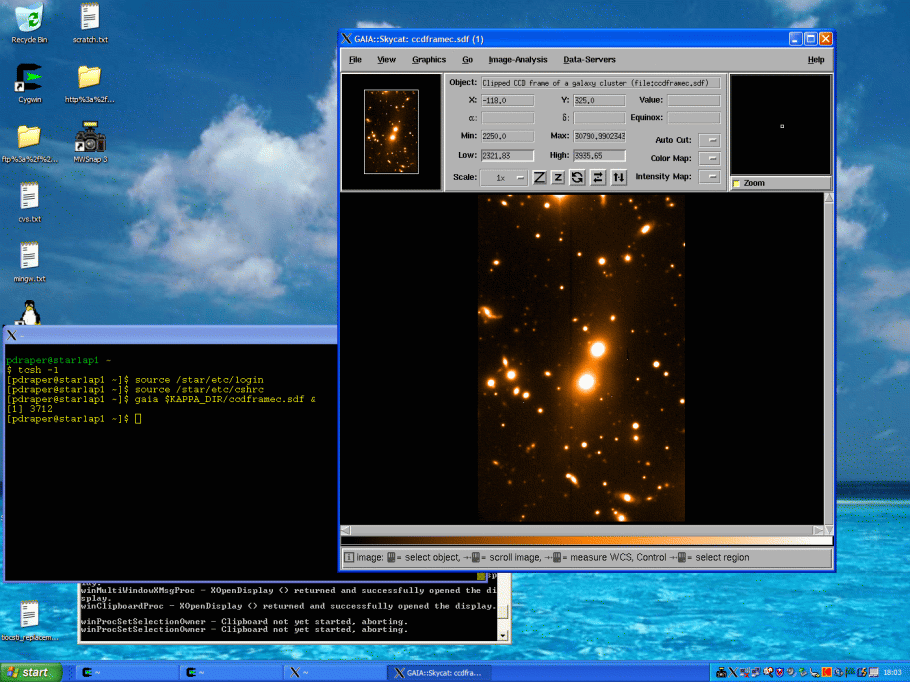
\includegraphics[width=0.8\linewidth]{starlinkcap}
	\caption{Interfaz del software Starlink}
	\label{fig:starlinkcap}
\end{figure}

\section*{Metodologia}
Una vez claro el marco de referencia en el que nos encontramos, se procede a iniciar el proceso de análisis de datos y exploración de tecnologías a utilizar. Para ello, nos dirigiremos en un principio a la página web de \href{https://magrathea.sdss.org/marvin/}{Marvin} con el fin de hallar una galaxia que nos resulte interesante para comenzar a analizarla. 

MaNGA (Mapping Nearby Galaxies at APO) es un estudio espectroscópico de campo integral de galaxias dentro de la cuarta generación del Sloan Digital Sky Survey (SDSS-IV). Mapeará la composición y cinemática del gas y las estrellas en 10.000 galaxias cercanas, utilizando 17 haces de fibras de diferentes tamaños. El objetivo de MaNGA es proporcionar nuevos conocimientos sobre la formación y evolución de galaxias, y ofrecer un punto de referencia local para los estudios actuales y futuros de alto desplazamiento al rojo.

Por ahora, tomaremos la galaxia \verb|manga 7495-6102| y descargaremos su cubo de datos \textbf{lineal}\footnote{Optamos por el cubo de datos lineal ya que el modelo logarítmico requiere de más técnica para poder manipularse} de la siguiente manera:
\begin{enumerate}
    \item En el inicio de la pagina click en el botón \textbf{Go to SkyServer}
    \item El la barra lateral derecha click al enlace \textbf{Explore}
    \item Al final de la pagina click en \textbf{MaNGA observation(s)}
    \item Click en \textbf{LIN Data Cube}
\end{enumerate}
A continuación, comenzará la descarga de nuestro cubo de datos. Este archivo que se descargará será del tipo \verb|.fits.gz|, lo que indica que nuestro archivo está comprimido, pero no será necesario descomprimirlo para el procesamiento.

\begin{figure}
    \centering
    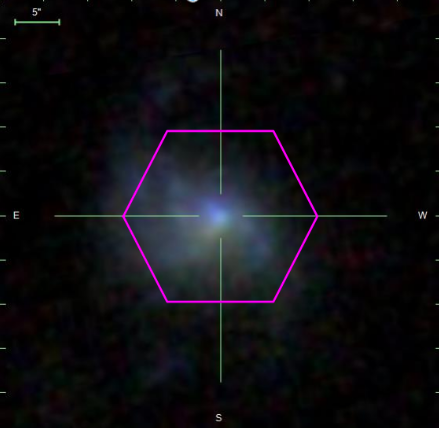
\includegraphics[width=0.8\linewidth]{manga-7495-6102.png}
    \caption{Galaxia 7495-6102 - MaNGA - https://magrathea.sdss.org/marvin/galaxy/7495-6102/}
    \label{fig:interfacemarvin}
\end{figure}
 
\subsection*{Procesamiento con Python}

Una vez descargado el cubo de datos, podremos analizarlo con la ayuda de \textbf{Python}, un lenguaje de programación interpretado multiplataforma, además de una librería llamada \textbf{Astropy}, enfocada en el análisis y procesamiento astronómico. También utilizaremos \textbf{numpy} y \textbf{matplotlib} para la graficación de nuestros datos.

\subsubsection*{Implementación en código}

Primero verificaremos cuáles son las dimensiones de nuestro cubo de datos.

\begin{lstlisting}[language=Python]
    from astropy.io import fits
    import numpy as np
    import matplotlib.pyplot as plt
    
    fits_file = './manga-7495-6102-LINCUBE.fits.gz' #ruta del archivo .fits
    hdul = fits.open(fits_file) #abre el archivo .fits
    flux = hdul["FLUX"].data #lee los datos de flujo
    print(flux.shape) #dimensiones del cubo de datos (espectral x espacial x espacial)
    #resultado: (6732, 54, 54)
\end{lstlisting}

El resultado del código anterior indica que tenemos un cubo de datos de 54×5454×54 (espacial) = 2916 spaxels, con una profundidad de 6732 espectros, dando un total de 19,630,512 voxels.
\begin{lstlisting}[language=Python]
    from astropy.io import fits
    import numpy as np
    import matplotlib.pyplot as plt
    import matplotlib.ticker as ticker
    fits_file = '../manga-7495-6102-LINCUBE.fits.gz'
    #ruta del archivo .fits
    hdul = fits.open(fits_file) #abre el archivo .fits
    flux = hdul["FLUX"].data #lee los datos de flujo
    print(flux.shape) #dimensiones del cubo de datos
    #(espectral x espacial x espacial)
    #el nmero de espectros es (6732, 54, 54)
    
    flg=plt.figure()
    ax = flg.add_subplot(111)
    ax.plot(flux[:,27,27])
    ax.set_ymargin(0.1)
    #ax.set_xlim(self.datacube.getData("WAVE")[0])
    ax.xaxis.set_major_formatter( ticker.FuncFormatter( lambda x, pos: '{}{}'.format('', str(int(x)+self.datacube.getData("WAVE")[0]))))
    ax.set_xlabel("Longitud de onda Å")
    ax.set_ylabel("Flujo [10-17 erg/cm2/s/Å]")
    ax.set_title("Galaxia: manga-7495-6102 \nSpaxel: 27,27") 
    
    #extrayendo un corte del cubo en la longitud de onda 900 a través de toda la imagen y aplicando log10 - devuelve una imagen  
    fig=plt.figure()
    bx=fig.add_subplot(111) 
    cx = bx.imshow(np.log10(flux[900,:,:]))
    
    plt.show() #muestra los gráficos
\end{lstlisting}

\begin{figure}
    \centering
    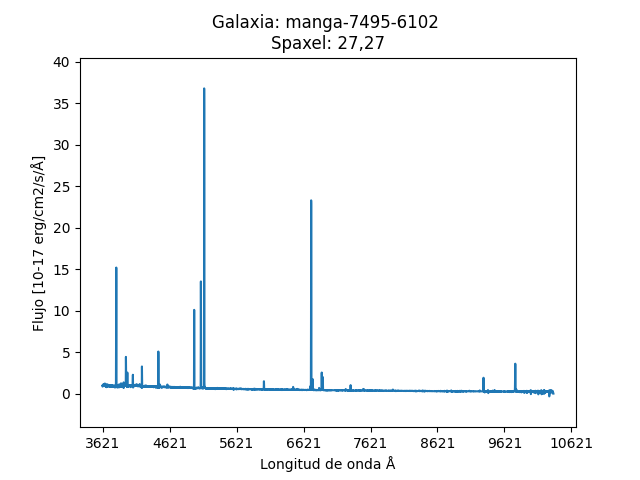
\includegraphics[width=1\linewidth]{espectro1_python.png}
    \caption{Espectro en (:, 27, 27)}
    \label{fig:espectro1_python}
\end{figure}
Al ejecutar este código se desplegarán dos ventanas: una gráfica con el espectro del spaxel \texttt{(espectro: todos, espacial: 27px, espacial: 27px)} \textbf{(Fig. 8)}, y una gráfica con la imagen de la galaxia en \texttt{(espectro: 900, espacial: todos, espacial: todos)} \textbf{(Fig. 9)}.

\begin{figure}
    \centering
    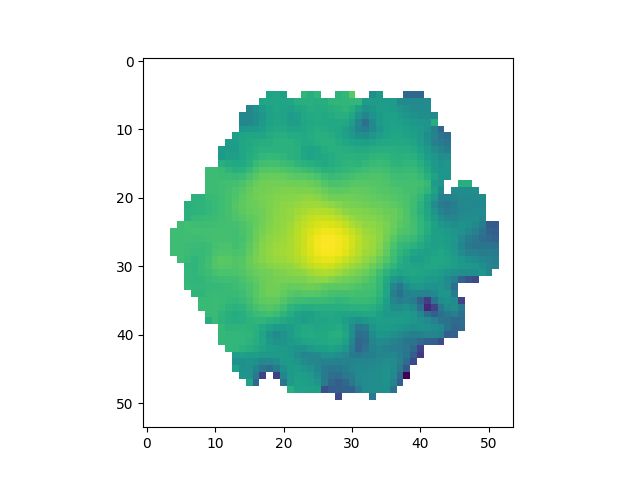
\includegraphics[width=1\linewidth]{imagen1_python.png}
    \caption{Imagen en (900, :, :) con logaritmo base 10 aplicado}
    \label{fig:imagen1_python}
\end{figure}

\subsubsection*{Ajuste de longitud de onda en los datos}

Dado que los datos de los espectros están situados en una longitud de onda específica y no comienzan en 0, debemos agregar al eje xx los datos que corresponden a las longitudes de onda específicas para cada espectro. Estos datos se encuentran dentro del mismo archivo .fits en el apartado "WAVE".

\subsubsection*{Ajuste de redshift o corrimiento al rojo}

Gracias al efecto Doppler, nuestros datos presentan un desfase en las longitudes de onda que nos son presentadas. Por lo tanto, debemos realizar otro ajuste a las longitudes de onda basándonos en la cantidad de corrimiento al rojo. Para ello, recurriremos al DAPall del SDSS, un resumen de las tablas finales de los resultados del MaNGA Data Analysis Pipeline (DAP), en el cual se encuentra la cantidad de redshift de nuestra galaxia en base al PLATEIFU.

Para ello se utilizará el siguiente código:

\begin{lstlisting}[language=Python]
    from astropy.io import fits
    import numpy as np 
    import matplotlib.pyplot as plt
    nombre_arch="./manga-7495-6102-LINCUBE.fits.gz"
    hdu=fits.open(nombre_arch)
    flujo = hdu["FLUX"].data
    print("Dimensiones: ",flujo.shape)
    hdu_catalog=fits.open( "./redshift_catalog/dapall-v3_1_1-3.1.0.fits")
    data_catalog=hdu_catalog[1].data
    ix=np.where(data_catalog["plateifu"] == "7495-6102") 
    redshift=data_catalog[ "nsa_z"][ix][0]
    longitud=hdu[ "WAVE"].data
    wave=longitud/(1.0 + redshift)
    fig=plt.figure()
    ax=fig.add_subplot(111)
    ax.plot(longitud, flujo[:,27,27]) 
    ax.plot(wave,flujo[:,27,27])
    plt.show()
\end{lstlisting}

Lo que nos da como resultado una gráfica con los dos espectros: el espectro observado (en azul) y el estado en reposo o rest frame (en naranja), ambos ya calibrados en la longitud de onda respectiva \textbf{Fig. 10}.

\begin{figure}
    \centering
    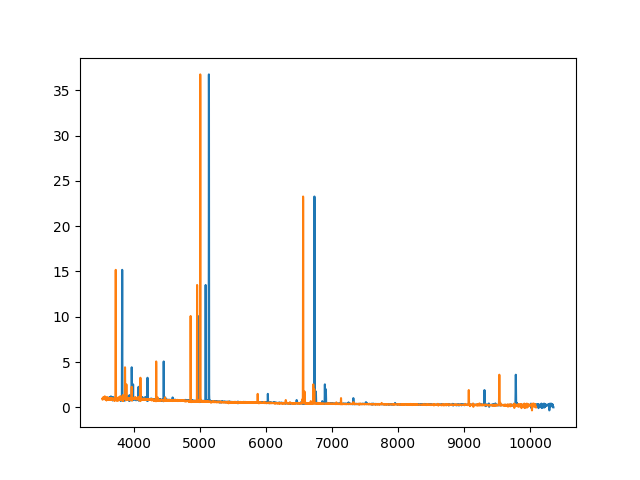
\includegraphics[width=1\linewidth]{redshift_ajuste.png}
    \caption{Ajuste de longitud de onda por redshift}
    \label{fig:redshift_ajuste}
\end{figure}

Para obtener una manipulación completa de los datos, me he basado en la información de la página del \href{https://data.sdss.org/datamodel/files/MANGA_SPECTRO_DATA/MJD5/sdR.html}{Modelo de Datos del SDSS}, en la que se especifican los apartados de un archivo \verb|.fits|.

\subsubsection*{Resultados}
Al finalizar este proceso, logré comprender cómo se observan los objetos celestes usando espectroscopía integral de campo, incluyendo la estructura de un archivo proveniente del MaNGA / SDSS. Exploré temas de física, computación y análisis de datos.

\subsection*{Creación de interfaz}
Con el fin de facilitar el uso de la implementación anterior, me propuse crear un entorno gráfico para esta. Entre las varias alternativas disponibles en Python, escogí \href{https://dearpygui.readthedocs.io/en/latest/}{Dearpygui}, ya que es una librería gráfica multiplataforma, dinámica, acelerada por GPU y fácil de usar; un kit de herramientas de interfaz de usuario (GUI) para Python. Dado que en esta ocasión se manejarán grandes volúmenes de datos y requerimos una interfaz de alto rendimiento, cabe mencionar que esta librería también permite crear gráficas o "plots", así que para la sección del espectro me tomé la libertad de usar la alternativa de Dearpygui.

El programa de visualización creado, al que he denominado InterVisor, permite abrir un nuevo archivo \verb|.fits|, \verb|.gz| o \verb|.fits.gz| desde el explorador de archivos con el botón \textbf{Open a new file}. Además, maneja un registro de los archivos abiertos con anterioridad; para ello está el botón \textbf{Recent files}. Para finalizar el programa, está la opción \textbf{Exit} \textbf{(Fig. 11-13)}.

\begin{figure}
    \centering
    
\includegraphics[width=1\linewidth]{menuprincipal1.png}
    \caption{Menu principal}
    \label{fig:menuprincipal1}
\end{figure}

\begin{figure}
    \centering
    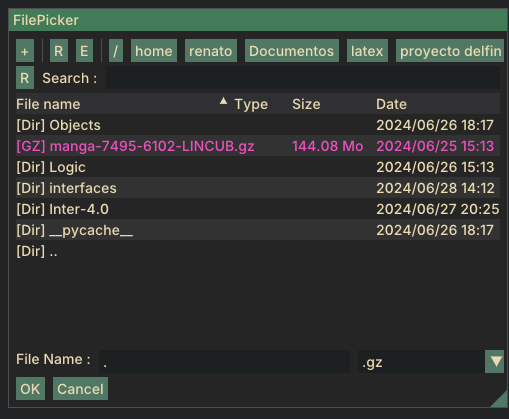
\includegraphics[width=1\linewidth]{file_explorer_visor.png}
    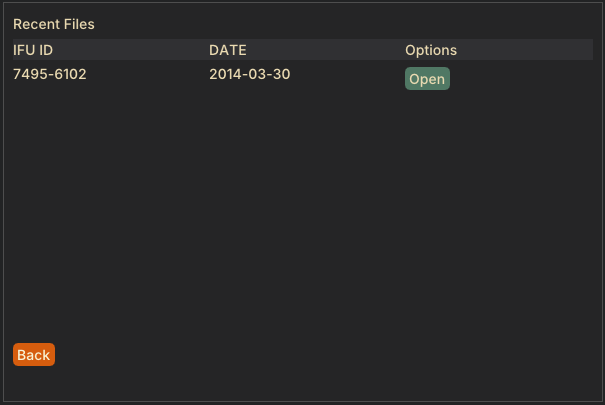
\includegraphics[width=1\linewidth]{recent_files.png}
    \caption{Archivos Recientes y Explorador de archivos}
    \label{fig:recent_files}
\end{figure}

Al abrir algún archivo se procede a la siguiente pantalla en la cual se presentan las diferentes opciones para procesar el archivo \textbf{Fig. 14}.

\begin{figure}
    \centering
    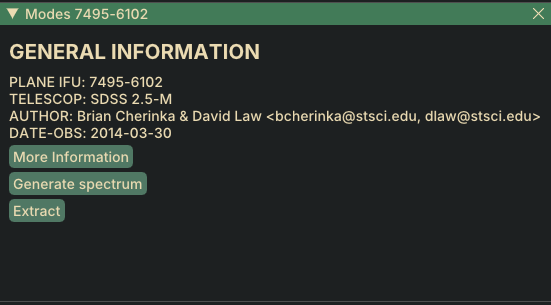
\includegraphics[width=1\linewidth]{modes.png}
    \caption{Ventana de modos de procesamiento.}
    \label{fig:modes}
\end{figure}

Actualmente, se cuentan con los siguientes modos de procesamiento:

\begin{enumerate}
\item \textbf{Visor de espectro:} En este apartado se permite escoger el spaxel (i, j) y el rango de longitud de onda en el que se desea ver el espectro \textbf{(Fig. 15)}.
\item \textbf{Extractor de imagen:} Después de ingresar una longitud de onda específica, se muestra la imagen del mapa. También está la opción de aplicar $log_{10}$ y $log_{2}$ \textbf{(Fig. 16)}.
\item \textbf{Más información:} Un apartado para observar más datos sobre el archivo \verb|.fits| \textbf{(Fig. 17)}.
\end{enumerate}

\begin{figure}
\centering
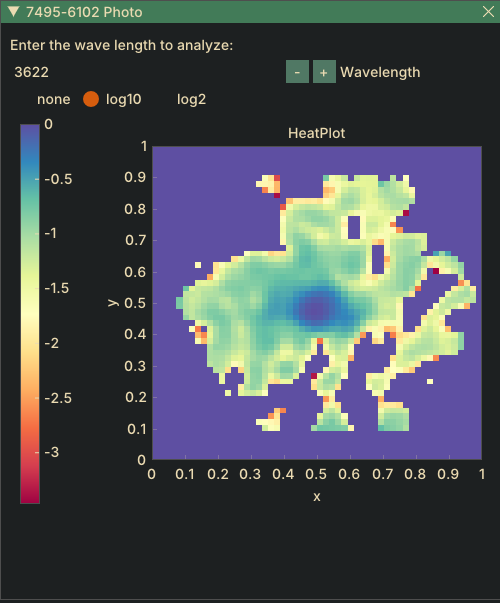
\includegraphics[width=0.8\linewidth]{VIsor_heatmap.png}
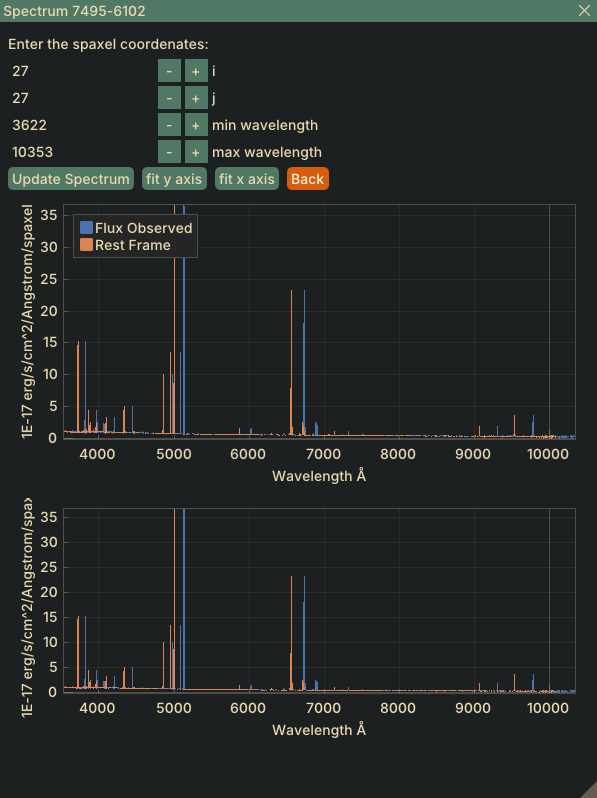
\includegraphics[width=0.8\linewidth]{spectrum_visor.png}
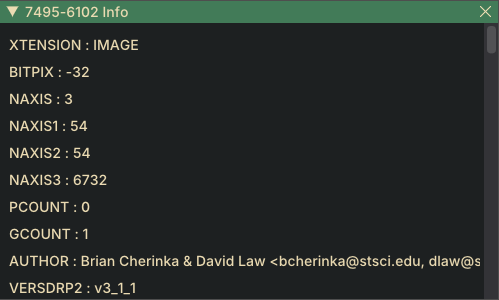
\includegraphics[width=0.8\linewidth]{moreinfo.png}
\caption{Opciones de visualización en el programa con interfaz gráfica.}
\label{fig
}
\end{figure}

\subsubsection*{Resultados}
Como resultado, se obtiene un programa con las operaciones básicas de visualización de archivos \verb|.fits| correspondientes al MaNGA. Utiliza las librerías Astropy, Numpy, Dearpygui y otras más. Además, permite la creación de rutinas de visualización consistentes y acoplables a otros métodos de análisis (visualización de espectros, mapas en una longitud de onda específica, información general del objeto observado).

\section*{Observación de Líneas de Emisión}

\subsection*{Lineas de emisión de interés}

\begin{enumerate}
  \item {[OII] \textbf{3727} Oxígeno ionizado (singly ionized)}
  \item {[NeIII] \textbf{3869} Neón ionizado (doubly ionized)}
  \item {Hδ \textbf{4102} Hidrógeno delta}
  \item {Hγ \textbf{4340} Hidrógeno gamma}
  \item {[OIII] \textbf{4363} Oxígeno ionizado (doubly ionized)}
  \item {[OIII] \textbf{4959} Oxígeno ionizado (doubly ionized)}
  \item {[OIII] \textbf{5007} Oxígeno ionizado (doubly ionized)}
  \item {HeI \textbf{5876} Helio neutro}
  \item {[OI] \textbf{6300} Oxígeno neutro}
  \item {[OI] \textbf{6364} Oxígeno neutro}
  \item {[NII] \textbf{6584} Nitrógeno ionizado (singly ionized)}
  \item {HeI \textbf{6678} Helio neutro}
  \item {[SII] \textbf{6717} Azufre ionizado (singly ionized)}
  \item {[SII] \textbf{6731} Azufre ionizado (singly ionized)}
  \item {HeI \textbf{7065} Helio neutro}
  \item {[ArIII] \textbf{7136} Argón ionizado (doubly ionized)}
  \item {[OII] \textbf{7320} Oxígeno ionizado (singly ionized)}
  \item {[ArIII] \textbf{7751} Argón ionizado (doubly ionized)}
\end{enumerate}

En base a estas líneas de emisión, se pueden obtener múltiples tipos de mapas:

\begin{itemize}
\item \textbf{Mapa de intensidad:} Área bajo la curva gausiana ajustada a los datos.
\item \textbf{Mapa cinético:} Movimiento de rotación de la galaxia.
\item \textbf{Mapa de temperatura:} Diferencias entre los anchos de las líneas de emisión.
\item \textbf{Estrellas antiguas:} Varianza entre las alturas del continuo.
\item \textbf{Razón iónica:} [SII]6717/[SII]6731[SII]6717/[SII]6731.
\end{itemize}

\subsection*{Mapa de Intensidad}

\textbf{Aclaraciones}

Antes de analizar los bloques de datos, he decidido realizar las siguientes operaciones:

\begin{enumerate}
\item \textbf{Discriminación de bloques de datos fuera del área observada:} Usando la función \texttt{numpy.all()}, se detecta si un arreglo de datos está lleno de ceros o si contiene valores infinitos no válidos para nuestro proceso. En estos casos, se procede a insertar \texttt{None} en la posición correspondiente en el arreglo bidimensional.
\item \textbf{Conversión de datos post-redshift:} Tras aplicar el redshift o corrimiento al rojo sobre el conjunto de datos de la longitud de onda del espectro, se procede a convertir estos datos a valores \textbf{int} para una mejor manipulación.
\end{enumerate}

Cuando analizamos una linea de emisión debemos de examinar toda la curva de emisión ya que hasta ahora hemos visto y analizado solo un corte en el cubo de datos a lo largo del espectro. Por ejemplo tenemos la linea de emisión de la \textbf{(Fig. 18)} donde podemos apreciar que la formacion de la linea de emisión en el fondo esta formada por un segmento del cubo de datos y no solo por una longitud de onda en especifico.

\textbf{Objetivo: } Hallar el area bajo la curva gausiana con ajuste a la linea de emision $n$. 

para iniciar hay que definir el método y nomenclatura que ocuparemos:
\subsubsection*{Extracción de datos de la linea de emisión}

\begin{enumerate}
  \item Definir el margen \( m \) usado para extraer el intervalo de datos referente a la línea de emisión \( n \), que comprende \( \text{flujo}[n-m:n+m] \).
  \item Definir un submargen \( p \) lateral para calcular la media del continuo a los costados de la línea de emisión.
  \item Calcular el FWHM (Full Width at Half Maximum) de la línea de emisión, lo que proporciona un sigma más preciso para la generación de una campana gaussiana.
  \item Ajustar una gausiana a los datos de la línea de emisión.
  \item Integrar el área bajo la curva gaussiana (sin incluir el área entre 0 y la media del continuo) y almacenar este dato en una matriz bidimensional.
  \item Generar la imagen con los datos de las líneas de emisión \( n \).
\end{enumerate}

Este proceso debe realizarse para cada píxel en la imagen del cubo de datos en cada una de las líneas de emisión que nos interesa analizar. De esta manera, obtendremos un mapa de líneas de emisión. Para generar la gausiana, utilizamos la siguiente fórmula:

$$
f(x) = a \cdot \exp\left( -\frac{(x - x_0)^2}{2\sigma^2} \right)
$$

Además, usamos la función \textbf{curve\_fit} de la librería \textbf{scipy.optimize} para ajustar la gausiana a los datos. El código utilizado se encuentra en mi repositorio de \href{https://github.com/renatosanz/delfin}{GitHub}.

Una vez claro el proceso para un píxel específico en el cubo de datos, podemos proceder a automatizar este proceso para cada uno de los píxeles en el cubo, y almacenar los datos en un arreglo bidimensional para finalmente generar una imagen (mapa) de líneas de emisión.

\begin{figure}
    \centering
    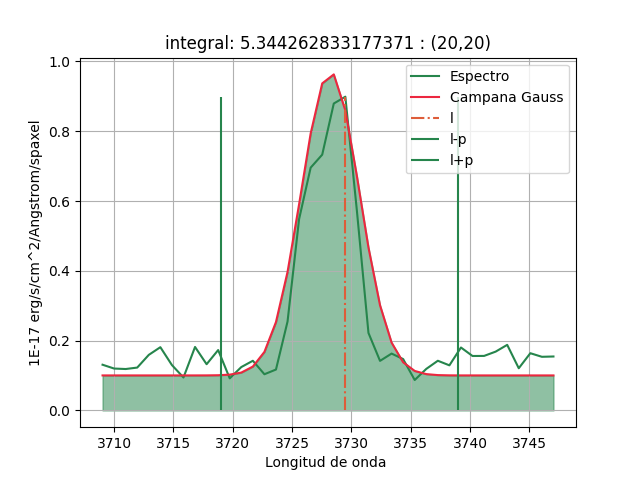
\includegraphics[width=1\linewidth]{extraccion_linea.png}
    \caption{Visualización del proceso de extracción de la intensidad de líneas de emisión.}
    \label{fig:extraccion_linea}
\end{figure}

\subsubsection*{Resultados}

Durante el proceso de generación de estos mapas de líneas de emisión, encontré dificultades para \textbf{calcular el FWHM}. En el momento de ajustar la campana de Gauss, me resultó complicada la forma en que debía obtener dicho valor. Después de investigar, encontré una explicación clara en esta \href{https://www.pulstec.net/what-is-full-width-at-half-maximum/}{página} (\cite{suzuki2023fwhm}).

De esta manera, obtuve resultados como los siguientes: imágenes con una gran cantidad de píxeles calculados y una barra de medición al costado. Además, en la \textbf{Fig. 18}, el área verde representa el valor de la integración de la campana de Gauss, el área naranja representa la zona que no debemos tomar en cuenta en este proceso, las barras laterales se interpretan como los submárgenes a partir de los cuales se calcula la media del continuo, y el intervalo central es la zona en la que se halla la información de la línea de emisión.

\begin{figure}
    \centering
    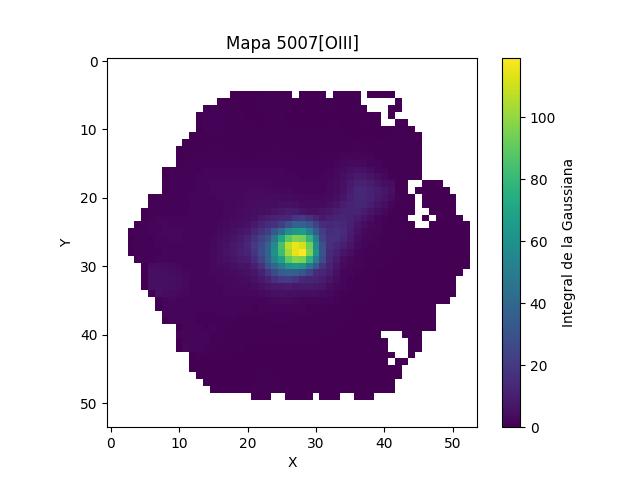
\includegraphics[width=0.8\linewidth]{../Codigos/extractorLineasEmision/imgs/imgs7495-6102_lines/img7495-6102_[OIII]_5007_.png}
    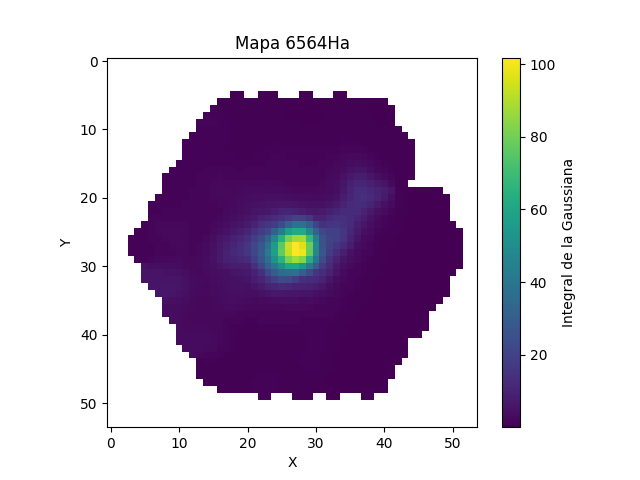
\includegraphics[width=0.8\linewidth]{../Codigos/extractorLineasEmision/imgs/imgs7495-6102_lines/img7495-6102_Ha_6564_.png}
    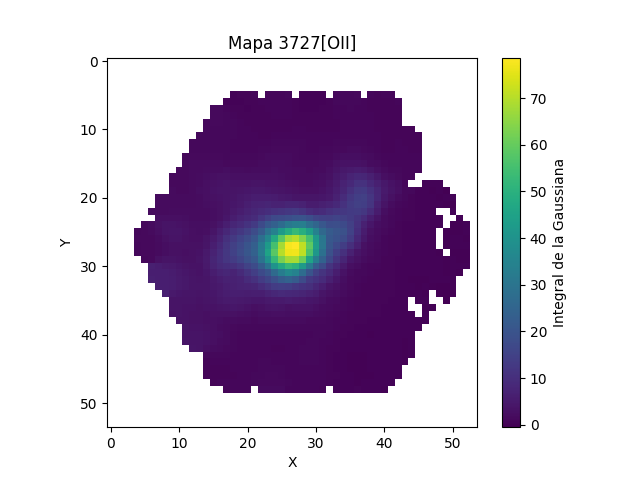
\includegraphics[width=0.8\linewidth]{../Codigos/extractorLineasEmision/imgs/imgs7495-6102_lines/img7495-6102_[OII]_3727_.png}
    \caption{PLATEIFU: 7495-6102}
    \label{fig:moreinfo}
\end{figure}

\newpage


\section*{Proyecto Final}

\subsection*{Diagramas de diagnóstico / BPT}
Los diagramas de diagnóstico ayudan a distinguir cual es la fuente de ionización del objeto observado (estrellas, núcleos activos de galaxias, choques, etc.).

\begin{figure}
  \begin{center}
    
\includegraphics[width=1\linewidth]{./diagrama_ejemplo.png}
  \end{center}
  \caption{Ejemplo visual de un diagrama de diagnóstico.}
  \label{fig:diagrama_profe}
\end{figure}

Como último proceso, se planea la generación de diagramas de diagnóstico, los cuales proporcionarán información sobre el objeto observado. Para esto, se debe realizar el siguiente proceso:
\begin{enumerate}
  \item Una vez obtenidas las líneas de emisión y almacenadas en un archivo \texttt{.fits}, procederemos con la integración de estos datos\footnote{Con integrar nos referimos a sumar todos los datos que conforman la imagen de la línea de emisión, pasando de una matriz bidimensional a un solo valor} de las líneas de emisión [NII] 6548, Ha 6564, Hb 4861, [OIII] 5007. Para la integración de la de losdatos creé una función que verifica si la misma locación en ambos flujos contiene datos o no. De ser cierto, se realiza la suma de los datos como se puede observar.
    \begin{lstlisting}[language=Python]
def integrar(flujo):
    suma = 0
    for i in flujo:
        if np.all(flujo == np.nan):
            continue
        for k in i:
            if not np.isnan(k):
                suma += k
    return suma


hdul_NII = open("fits7495-6102_[NII]_6548_.fits")
hdul_Ha = open("fits7495-6102_Ha_6564_.fits")
hdul_Hb = open("fits7495-6102_Hb_4861_.fits")
hdul_OIII = open("fits7495-6102_[OIII]_5007_.fits")

integradoNII = integrar(flujoNII)
integradoHb = integrar(flujoHb)
integradoHa = integrar(flujoHa)
integradoOIII = integrar(flujoOIII)
    \end{lstlisting}
    
  \item A continuación, tomamos estos datos y realizamos las operaciones \(\log_{10}(\text{NII}/\text{Ha})\) y \(\log_{10}(\text{OIII}/\text{Hb})\).
    \begin{lstlisting}[language=Python]
NIIdivHa = integradoNII / integradoHa
OIIIdivHb = integradoOIII / integradoHb
Log10NIIdivHa = np.log10(integradoNII / integradoHa)
Log10OIIIdivHb = np.log10(integradoOIII / integradoHb)
    \end{lstlisting}
  \item Para determinar si nuestra galaxia contiene formación estelar, usaré las funciones \textbf{(4)} \(0.61 / (\log_{10}(\text{NII}/\text{Ha}) - 0.05) + 1.3\) (Kauffmann+03 line) y \textbf{(5)} \(0.61 / (\log_{10}(\text{NII}/\text{Ha}) - 0.47) + 1.19\) (Kewley+01 line) del artículo \cite{2006MNRAS.372..961K}, las cuales graficaré sobre el plano al mismo tiempo que los datos obtenidos anteriormente.
    \begin{lstlisting}[language=Python]
X = np.linspace(-2, 0.049, 100)
Y = 0.61 / (X - 0.05) + 1.3
ax.plot(X, Y, c="k", linestyle="--", label="Y = 0.61/[X-0.05]+1.3")

X1 = np.linspace(-2, 0.46, 1900)
Y1 = 0.61 / (X1 - 0.47) + 1.19
ax.plot(X1, Y1, label="Y1 = 0.61/[X1-0.47]+1.19")

ax.plot(
    Log10NIIdivHa,
    Log10OIIIdivHb,
    "ro",
)
    \end{lstlisting}
\end{enumerate} 

Este proceso lo he repetido con los cubos de datos manga-7495-6102, manga-8988-6104 y manga-7960-3704 de los cuales se obtieron resultados que reflejan formación estelar dentro de ellos. 

\begin{figure}[h!]
    \centering
    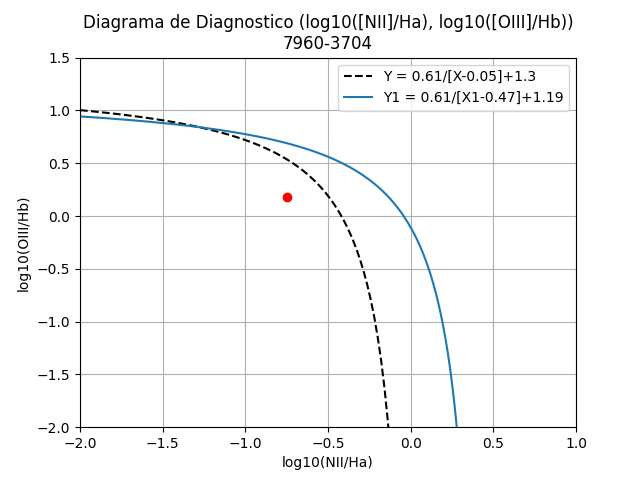
\includegraphics[width=1\linewidth]{../Codigos/diagramasDeDiagnostico/diagrama7960-3704.png}
    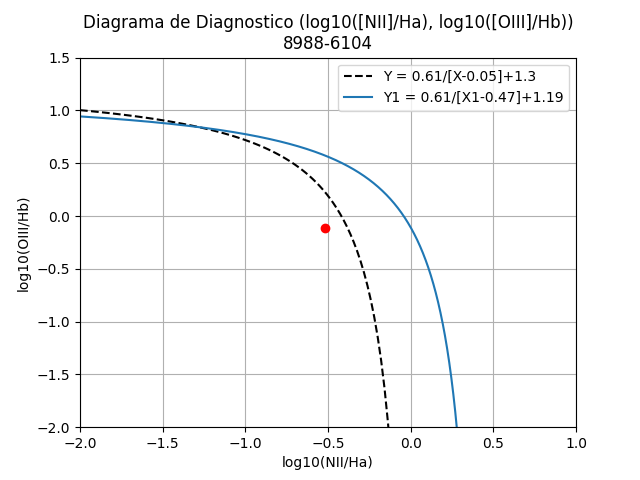
\includegraphics[width=1\linewidth]{../Codigos/diagramasDeDiagnostico/diagrama8988-6104.png}
    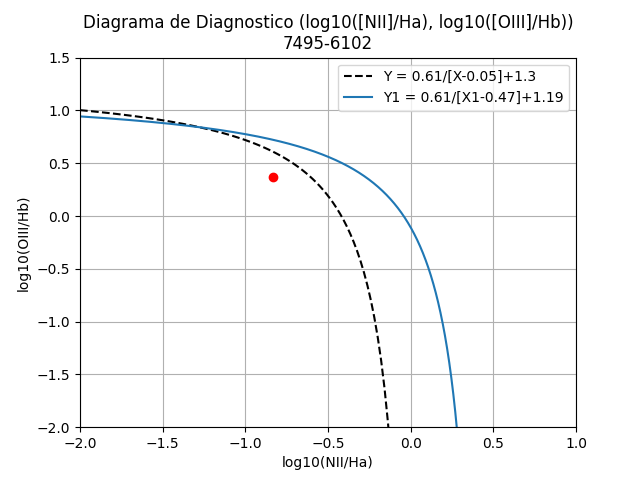
\includegraphics[width=1\linewidth]{../Codigos/diagramasDeDiagnostico/diagrama7495-6102.png}
    \caption{Diagramas BPT de las galaxias manga-7495-6102, manga-8988-6104 y manga-7960-3704}
    \label{fig:recent_files}
\end{figure}


\subsection*{Diagrama en resolución completa}
Para seguir avanzando en nuestro objetivo de analizar la fuente ionización se propone la generación del anterior diagrama BPT a resolución completa ($nxn$, con $n$ igual al tamaño del cubo de datos en las dimensiones espaciales).

Para lograr un analisis certero de las lineas de emision en cada pixel del cubo de datos se utilizaron las lineas de emisión del proceso anterior pero procesadas de una manera diferente.


\begin{enumerate}
  \item Primero se obtienen los flujos de las lineas de emision:
  \begin{lstlisting}[language=Python]
plateifu = "7960-3704"

hdul_NII = open(
    f"fits{plateifu}_[NII]_6548_.fits"
)
hdul_Ha = open(
    f"fits{plateifu}_Ha_6564_.fits"
)

hdul_Hb = open(
    f"fits{plateifu}_Hb_4861_.fits"
)
hdul_OIII = open(
    f"fits{plateifu}_[OIII]_5007_.fits"
)
  \end{lstlisting}
  \item Despues mediante una función me aseguro de que los 4 flujos tengan datos en la misma locacion para tener coherecia en los resultados. Despues procedo a realizar las diviciones de los datos de manera individual y guardando los datos dentro de un arreglo para cada uno de los procesos (\(\log_{10}(\text{NII}/\text{Ha})\) y \(\log_{10}(\text{OIII}/\text{Hb})\)) que posteriormente seran graficados.
  \begin{lstlisting}[language=Python]
def integracionPar(f1, f2, f3, f4):
    f = f1.shape
    datos_f1 = []
    datos_f2 = []
    datos_f3 = []
    datos_f4 = []
    for i in range(f[0]):
        if np.all(f1[i] == np.nan) or np.all(f2[i] == np.nan):
            continue
        for k in range(f[1]):
            if (
                not np.isnan(f1[i][k])
                and not np.isnan(f2[i][k])
                and not np.isnan(f3[i][k])
                and not np.isnan(f4[i][k])
            ):
                datos_f1.append(f1[i][k])
                datos_f2.append(f2[i][k])
                datos_f3.append(f3[i][k])
                datos_f4.append(f4[i][k])
    f1divf2 = []
    f3divf4 = []

    print(len(datos_f1), len(datos_f2), len(datos_f3), len(datos_f4))
    for i in range(len(datos_f1)):
        if (
            datos_f1[i] != 0
            and datos_f2[i] != 0
            and datos_f3[i] != 0
            and datos_f4[i] != 0
        ):
            try:
                div1_2aux = log10(datos_f1[i] / datos_f2[i])
                div3_4aux = log10(datos_f3[i] / datos_f4[i])
                print(div1_2aux)
                print(div3_4aux)
                f1divf2.append(div1_2aux)
                f3divf4.append(div3_4aux)
            except Exception as e:
                pass

    return f1divf2, f3divf4

flujoNII = hdul_NII[0].data
flujoHa = hdul_Ha[0].data
flujoHb = hdul_Hb[0].data
flujoOIII = hdul_OIII[0].data

Log10NIIdivHa, Log10OIIIdivHb = integracionPar(flujoNII, flujoHa, flujoOIII, flujoHb)
  \end{lstlisting}
  \item Finalmente graficamos los resultados:
  \begin{lstlisting}
    flg = plt.figure()
ax = flg.add_subplot(111)
ax.set_title(
    f"Diagrama de Diagnostico (log10([NII]/Ha), log10([OIII]/Hb))\nNube de puntos : {plateifu}"
)
ax.set_xlabel("log10(NII/Ha)")
ax.set_ylabel("log10(OIII/Hb)")


X = np.linspace(-2, 0.049, 100)
Y = 0.61 / (X - 0.05) + 1.3
ax.plot(X, Y, c="k", linestyle="--", label="Y = 0.61/[X-0.05]+1.3")

X1 = np.linspace(-2, 0.46, 1900)
Y1 = 0.61 / (X1 - 0.47) + 1.19
ax.plot(X1, Y1, label="Y1 = 0.61/[X1-0.47]+1.19")

ax.set_xlim(-2, 1)  # Establece los límites del eje x
ax.set_ylim(-2, 1.5)  # Establece los límites del eje y

ax.plot(Log10NIIdivHa, Log10OIIIdivHb, "ro", markersize=1)
plt.grid()
plt.legend()
plt.show()
  \end{lstlisting} 
\end{enumerate}

Como resultado, se obtienen nubes de puntos que reflejan la fuente de ionización de dichos píxeles en el cubo. De la misma forma, se puede inferir que la fuente de ionización de cada objeto es directamente proporcional a la cantidad de puntos en el área bajo la curva de Kauffmann, tal como se observa en los resultados. Cabe mencionar que los datos obtenidos de este método son relativamente nuevos en el mundo del procesamiento de cubos de datos, por lo que no se han establecido referentes para delimitar comportamientos específicos como sí los tenemos en los diagramas BPT convencionales, como las funciones de Kauffmann y Kewley para la ubicación de fuentes de ionización.

\begin{figure}[h!]
    \centering
    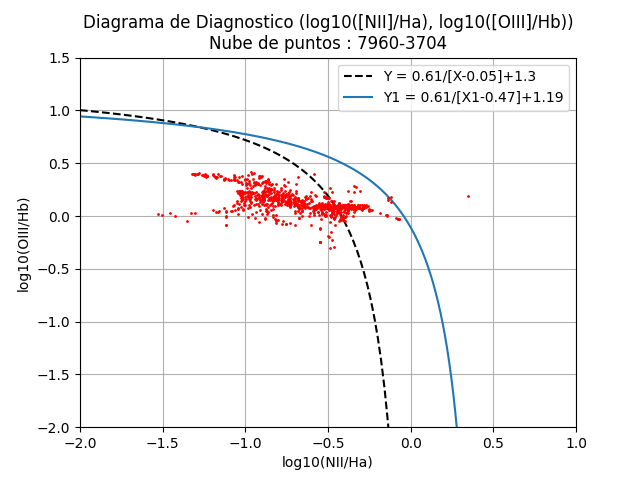
\includegraphics[width=1\linewidth]{../Codigos/diagramasDeDiagnostico/diagrama7960-3704_fullres.png}
    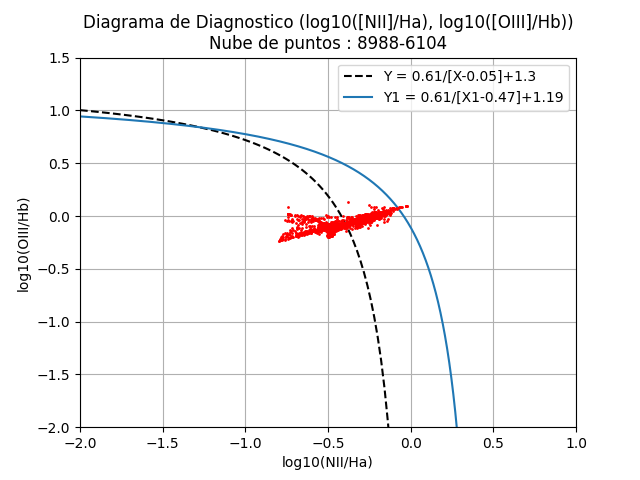
\includegraphics[width=1\linewidth]{../Codigos/diagramasDeDiagnostico/diagrama8988-6104_fullres.png}
    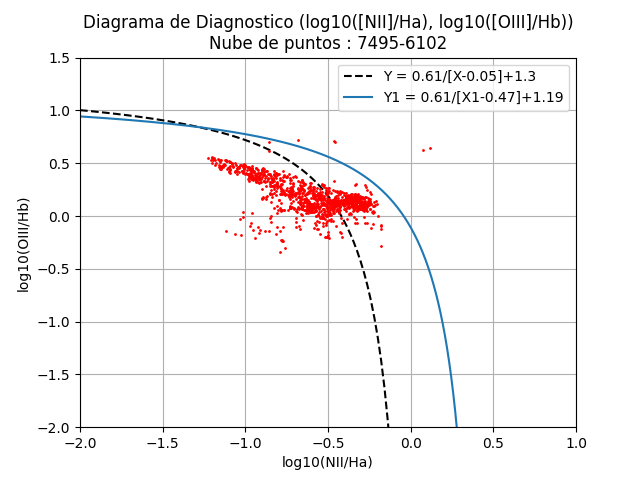
\includegraphics[width=1\linewidth]{../Codigos/diagramasDeDiagnostico/diagrama7495-6102_fullres.png}
    \caption{Diagramas BPT de las galaxias manga-7495-6102, manga-8988-6104 y manga-7960-3704 a resoluciones completas}
    \label{fig:recent_files}
\end{figure}

\section*{Conclusiones}
Durante la estancia se trataron temas de interés como la espectroscopía integral de campo, el manejo de archivos .fits y la creación de rutinas de visualización para cubos de datos provenientes del MaNGA. Esto estuvo orientado a la ubicación de formación estelar usando los diagramas BPT.

No puedo negar que estos temas son bastante complicados desde el punto de vista físico-matemático. Sin embargo, en el área de la programación y análisis de datos di todo lo que pude para obtener un producto terminado y listo para usarse, como lo es *InterVisor*. Este no está en su forma final, ya que en los siguientes meses estaré estudiando más opciones y mejoras que pueda hacer al sistema, tales como extracción de mapas de cinética, visualización 3D de la galaxia en cuestión o extracción de mapas de temperaturas.

Reflexionando sobre los resultados obtenidos del análisis a resolución completa, propongo lo siguiente. Si observamos la morfología de las nubes de puntos, se notan ciertos puntos lejos de la multitud. Estos puntos podrían reflejar la presencia de un AGN o agujero negro supermasivo, el cual, si bien no es la principal fuente de ionización, se puede observar dentro de estos datos. Un ejemplo de este comportamiento lo encontramos en el resultado del \textbf{manga-7495-6102}.

Para finalizar, quiero agradecer a mi asesor Jesús López Hernández, quien me introdujo a la astronomía desde un punto de vista computacional. Durante aproximadamente seis semanas aprendí bastante sobre el proceso detrás de los estudios interestelares, tanto de forma histórica, teórica como práctica.


\section*{Definiciones}
\begin{description}[style=nextline]
  \item[pixel] Un píxel se refiere a un píxel físico del detector que es leído por una serie de dispositivos electrónicos.
  \item[spaxel] Un spaxel (píxel espacial) se refiere a un elemento espacial de un cubo de datos reconstruido.
  \item[voxel] Un voxel (píxel volumétrico) se refiere a un elemento de volumen (espacial × espacial × espectral) de un cubo de datos. 
  \item[redshift] El desplazamiento al rojo, como lo indica su nombre, ocurre cuando las ondas de luz se estiran debido al efecto Doppler y tienden hacia la región roja del espectro.
  \item[FWHM] La anchura completa a la mitad de la altura (FWHM, por sus siglas en inglés) es una medida del ancho de una distribución de intensidad en el punto donde la intensidad es máxima. A menudo se utiliza para determinar el ancho de una línea espectral o el rango de longitudes de onda en luz monocromática. 
  \item[pársec] Unidad de medida de distancia utilizada en astronomía, equivalente a aproximadamente 3.26 años luz.
  \item[SDSS] El \textit{Sloan Digital Sky Survey} es uno de los proyectos de investigación astronómica más grandes jamás emprendidos. Su objetivo es expandir el conocimiento sobre la evolución y estructura del espacio, y la formación de estrellas y galaxias.
  \item[MaNGA] \textit{Mapping Nearby Galaxies at APO} es un estudio espectroscópico de campo integral de galaxias dentro del Sloan Digital Sky Survey de cuarta generación (SDSS-IV) \cite{weijmans2015manga}.
  \item[Unidad Astronómica / au] La unidad astronómica de distancia es una unidad de longitud utilizada en astronomía para las dimensiones típicas del Sistema Solar y se define como 1 au igual a exactamente 149,597,870.7 metros.
  \item[S/N] La relación señal-ruido (SNR, Signal-to-Noise Ratio) mide qué tan bien se mide un objeto. Valores típicos: \\
  S/N = 2-3: objeto apenas detectado \\
  S/N = 10: podemos comenzar a hacer mediciones \\
  S/N = 100: medición excelente. \\
  \item[Archivos .fits] FITS (Flexible Image Transport System) es el formato de datos más utilizado en astronomía para transportar, analizar y archivar datos. FITS no es solo un formato de imagen (como JPG o GIF), sino que está diseñado principalmente para almacenar conjuntos de datos científicos que constan de matrices multidimensionales (imágenes) y tablas bidimensionales organizadas en filas y columnas de información.
  \item[Diagramas BPT] Los diagramas BPT (llamados así por "Baldwin, Phillips & Terlevich") son un conjunto de diagramas de líneas de emisión nebular utilizados para distinguir el mecanismo de ionización del gas nebular. La versión más famosa muestra [NII]6584/Hα versus [OIII]5007/Hβ \cite{1981PASP...93....5B}.
\end{description}

\printbibliography

\end{document}
